\documentclass[dvipdfmx]{standalone}
\usepackage{tikz}
\usetikzlibrary{positioning}
\usetikzlibrary{patterns}
\usetikzlibrary{intersections, calc}

\begin{document}
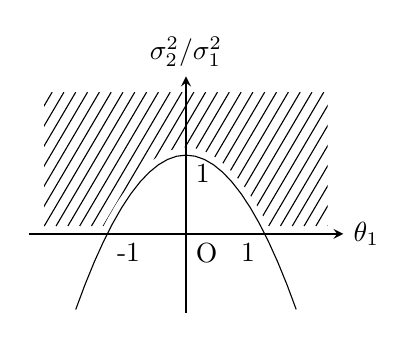
\begin{tikzpicture}
  \draw[->, >=stealth,semithick] (-2,0)--(2,0)node[right]{$\theta_1$}; %x軸
  \draw[->, >=stealth,semithick] (0,-1)--(0,2)node[above]{$\sigma_2^2/ \sigma_1^2$}; %y軸
  \draw (0,0)node[below right]{O}; %原点
  \draw[domain=-1.4:1.4] plot(\x, -\x*\x+1);

  \begin{scope}
    \clip (-1.8, 1.8)--(-1.8, 0)--(-1.1, 0.1)
          --plot[domain=-1.51:1.51](\x, -0.91*\x*\x + 1.1)
          --(1.1, 0.1)--(1.8, 0)--(1.8, 1.8);
    \foreach \t in {-20,-19,...,13}{
      \draw (0.15*\t, 0.1) -- (0.15*\t + 1.0, 1.8);
    }
  \end{scope}
  \draw (-1,0)node[below right]{-1};
  \draw (1,0)node[below left]{1};
  \draw (0,1)node[below right]{1};
\end{tikzpicture}
\end{document}
